\documentclass[cjk,slidestop,compress,mathserif,blue]{beamer}
%dvipdfm选项是关键,否则编译统统通不过
%beamer的颜色选项定义的是导航条和标题的颜色(即关键词structure的颜色)

%%%%%%%%%%%%%%%%仅限于XeTeX可使用的宏包%%%%%%%%%%%%%%%%%%%%%%%%%%%%
\usepackage{fontspec,xunicode,xltxtra,beamerthemesplit}
%\usepackage{beamerthemesplit}
\usepackage{xeCJK}
\setCJKmainfont[BoldFont=黑体, ItalicFont=楷体, BoldItalicFont=仿宋]{黑体}
%\setsansfont[Mapping=tex-text]{Adobe 黑体 Std}
%如果装了Adobe Acrobat,可在font.conf中配置Adobe字体的路径以使用其中文字体
%也可直接使用系统中的中文字体如SimSun,SimHei,微软雅黑 等
%原来beamer用的字体是sans family;注意Mapping的大小写,不能写错

%%%%%%%%   确定标题和导航条结构的框架     %%%%%%%%%%%%
\usepackage{beamerthemeshadow}                       %
%\usepackage{beamerthemeclassic}%导航条色与背景色一致%
%%%%%%%%%%%%%%%%%%%%%%%%%%%%%%%%%%%%%%%%%%%%%%%%%%%%%%
\setbeamerfont{roman title}{size={}}
%\usepackage{CJK} % CJK 中文支持                                  %
\usepackage{amsmath,amsthm,amsfonts,amssymb,bm}
\usepackage{mathrsfs}
\usepackage{xcolor}                                        %使用默认允许使用颜色
\usepackage{hyperref} 
\usepackage{graphicx}
\usepackage{subfigure}           %图片跨页
\usepackage{animate}		 %插入动画
\usepackage{caption}
\captionsetup{font=footnotesize}

%\usepackage[version=3]{mhchem}		%化学公式
\usepackage{chemfig}		%化学公式

\usepackage{multirow}
\usepackage{makecell}		%允许单元格内换行

\usepackage[dvipdfmx]{movie15_dvipdfmx} %插入视频
%\usepackage{handoutWithNotes}		%(讲义)在打印PPT的时候会留出给每一页做注释的部分
%\pgfpagesuselayout{1 on 1 with notes landscape}[a4paper,border shrink=5mm]

%\usepackage[numbers,sort&compress]{natbib} %紧密排列             %
\usepackage[sectionbib]{chapterbib}        %每章节单独参考文献   %
\usepackage{hypernat}                                                                         %
%\usepackage[dvipdfm,bookmarksopen=true,pdfstartview=FitH,CJKbookmarks]{hyperref}		%
\hypersetup{bookmarksnumbered,colorlinks,linkcolor=brown,citecolor=blue,urlcolor=red}         %
%参考文献含有超链接引用时需要下列宏包,注意与natbib有冲突        %
%\usepackage[dvipdfm]{hyperref}                                  %
%\usepackage{hypernat}                                           %
\newcommand{\upcite}[1]{\hspace{0ex}\textsuperscript{\cite{#1}}} %

%\useoutertheme{smoothbars}
\useinnertheme[shadow=true]{rounded}
\usetheme{Berkeley}                                          %主题式样
%\usetheme{Luebeck}

\usecolortheme{lily}                                        %颜色主题式样

\usefonttheme{professionalfonts}                           %字体主题样式宏包

%\beamertemplatetransparentcoveredhigh                      %使所有被隐藏的文本高度透明
\beamertemplatetransparentcovereddynamicmedium             %使所有被隐藏的文本完全透明,动态,动态的范围很小
\mode<presentation>
%\beamersetaveragebackground{gray}                          %设置背景颜色(单一色) 
\beamertemplateshadingbackground{green!10}{red!5}         %设置背景颜色(渐变色)

%在指定位置精确放置logo
\usepackage{tikz}
\usepackage{beamerfoils}
\usepackage{pgf}
\logo{\pgfputat{\pgfxy(9.99,0.00)}{
\includegraphics[height=0.75cm,viewport=5 2 520 120,clip]{Figures/BCC_logo-1.png}}}
%\logo{\pgfputat{\pgfxy(10.45,0.00)}{
\includegraphics[height=0.65cm,viewport=6.5 39 264 102,clip]{Figures/BCC_logo-2.jpg}}}
%\logo{\pgfputat{\pgfxy(11.68,0.15)}{
\includegraphics[height=1.01cm,viewport=0 0 140 120,clip]{Figures/BCC_logo-1.png}}\pgfputat{\pgfxy(10.502,-0.218)}{
\includegraphics[height=0.369cm,viewport=140 0 540 120,clip]{Figures/BCC_logo-1.png}}}
%\logo{\pgfputat{\pgfxy(11.38,0.24)}{
\includegraphics[height=1.50cm,viewport=26 12 440 420,clip]{Figures/BCC_logo.jpg}}}

%\logo{\pgfputat{\pgfxy(10.28,0.00)}{
\includegraphics[height=0.95cm,viewport=0 0 1100 360,clip]{Figures/Logo_Gainstrong.png}}}
%\logo{\pgfputat{\pgfxy(11.68,0.15)}{
\includegraphics[height=0.95cm,viewport=0 0 510 360,clip]{Figures/Logo_Gainstrong.png}}\pgfputat{\pgfxy(10.333,-0.195)}{
\includegraphics[height=0.35cm,viewport=530 70 1100 218,clip]{Figures/Logo_Gainstrong.png}}}
%\MyLogo{
%	\pgfputat{\pgfxy(-50,-50)}{\pgfbox[right,base]{
\includegraphics[height=1cm]{Figures/BCC_logo-1.png}}}

%logo作为背景放置
%\setbeamertemplate{background}{
%	\pgfputat{\pgfxy(6.5,-0.5)}{\pgfbox[left,top]{\pgfimage[height=1.1cm]{Figures/BCC_logo-1.png}}}}

%\logo{}									%不显示logo

\begin{document}
\begin{document}
%\begin{CJK*}{GBK}{song}
%\begin{CJK*}{GBK}{kai}
%beamer下不能用\songyi、\zihao等命令!
%\graphicspath{Figures/}

%-------------------------------PPT Title-------------------------------------
\title{基于甲烷燃烧催化机理的\\材料计算自动流程设计}
%-----------------------------------------------------------------------------

%----------------------------Author & Date------------------------------------
\author[]{北京市计算中心\;云平台\:姜骏}
	
\institute[]{}
%\date{2013.09.10}
\date{\textrm{2017.07.26}}
\frame
{	
	\frametitle{\footnotesize{\textcolor{orange}{\textrm{2018~}年度“青年骨干计划”}}}
\titlepage
}
%-----------------------------------------------------------------------------

%------------------------------------------------------------------------------列出全文 outline ---------------------------------------------------------------------------------
\section*{}
\frame[allowframebreaks]
{
  \frametitle{Outline}
%  \frametitle{\textcolor{mycolor}{\secname}}
  \tableofcontents%[current,currentsection,currentsubsection]
}
%在每个section之前列出全部Outline
%类似的在每个subsection之前列出全部Outline是\AtBeginSubsection[]
\AtBeginSection[]
{
  \frame<handout:0>
  {
    \frametitle{Outline}
%全部Outline中,本部分加亮
    \tableofcontents[current,currentsection]
  }
}

%------------------------------------------------------------------------------PPT main Body------------------------------------------------------------------------------------
\small
%\section{个人信息}
\frame
{
	\frametitle{个人信息}
\begin{minipage}[b]{0.72\linewidth}
	姓~名\hspace{15pt}姜~骏\hspace{45pt}出生年月\hspace{15pt}1978.12\\
	\vskip
	学~位\hspace{15pt}理学博士\hspace{25pt}专业方向\hspace{15pt}物理化学\\
	\vspace*{15pt}
\end{minipage}
\hfill
\begin{minipage}[b]{0.26\linewidth}
	\vspace{20pt}
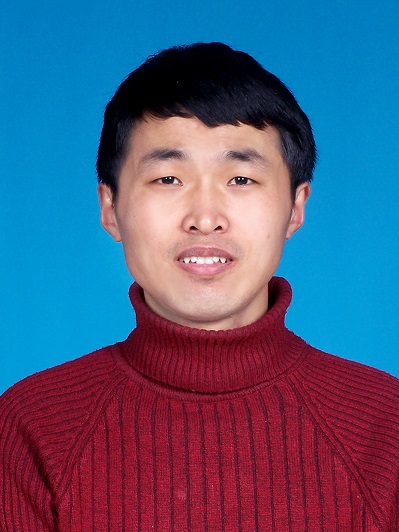
\includegraphics[height=0.8in]{Figures/Person_Photo.JPG}\\
\end{minipage}
	当前从事专业\hspace{10pt}材料计算软件开发与金属材料计算\\
	\vspace*{15pt}
	工作单位及部门\hspace{5pt}北京市计算中心\hspace{5pt} 云平台事业部\\
	\vspace*{15pt}
	\textcolor{magenta}{承担课题}\hspace{5pt}“材料基因工程关键技术与支撑平台”重点专项
}

\section{项目背景}
\frame
{
	\frametitle{项目背景}
	\begin{itemize}
		\item 天然气储量丰富、热效率高、价格低廉、污染较小。但天然气主要成分甲烷直接燃烧,温度高达~1600$^{\circ}\mathrm{C}$左右,在没有催化剂的情况下,在空气中燃烧生成氮氧化物等物质,对环境造成一定的污染。通过催化剂作用,降低燃料的起燃温度和燃烧的峰值温度,提高甲烷燃烧利用率,减少大气污染物生成
		\item 在催化剂存在时,甲烷的多相催化氧化反应和自由基反应同时发生,在~377$\sim$877$^{\circ}\mathrm{C}$的温度区间内两者均起作用,这对研究催化反应的反应机理带来了很大的困难
		\item 利用第一原理计算工具,有可能从理论角度探索甲烷燃烧催化机理,为有关实验研究提供辅助和支持;~在研的“材料基因工程关键技术与支撑平台”任务已开发了支持金属材料计算平台,为催化材料计算提供了经验和积累
	\end{itemize}

}

\section{项目规划}
\frame
{
	\frametitle{项目目标}
\begin{minipage}[b]{0.58\linewidth}
	\begin{itemize}
		\setlength{\itemsep}{15pt}
		\item 针对第一原理计算特点,开发适应甲烷催化燃烧机理研究的自动流程计算平台并程序化
		\item 自动流程计算平台将包括结构建模的可视化,计算流程的自动化,结果数据分析的可视化
		\item 将开发的自动流程应用于六铝酸盐系列(\chemfig{MAl_{12}O_{19}})甲烷燃烧催化剂计算
	\end{itemize}
\end{minipage}
\hfill
\begin{minipage}[b]{0.38\linewidth}
\begin{figure}[t!]
\centering
\includegraphics[height=1.8in]{Figures/MP-type_Cat.png}\\
\label{fig:MP-type_Cat}
\caption{\footnotesize \textrm{The Structure of \chemfig{MAl_{12}O_{19}}.}}%
\end{figure} 
\end{minipage}
}

\frame
{
	\frametitle{技术路线}
	\begin{itemize}
		\setlength{\itemsep}{15pt}
		\item 自动流程计算平台主体框架的实现,将基于“材料基因工程”项目开发的\chemfig{Ni}-基单晶高温合金模拟的软件平台开发,适应催化机理研究,该平台是基于\textrm{Python~}开发的,核心的第一原理计算将采用\textrm{Gaussian}/\textrm{VASP}/\textrm{ADF}中的一种或几种
		\item 材料计算的可视化主要包括输入模型和计算结果可视化,在本平台的开发中,可视化主要通过集成开源的结构可视化工具如\textrm{GSview~}、\textrm{Xcrysten~}和\textrm{VESTA}和数据可视化绘图工具如\textrm{Gnuplot}、\textrm{Pymatlib~}模块(\textrm{Python~}自带)实现
		\item 该计算平台针对甲烷燃烧催化研究的典型应用,通过对六铝酸盐系列(\chemfig{MAl_{12}O_{19}})催化甲烷燃烧过程的模拟,探索甲烷燃烧的催化机理\\
	\end{itemize}
}

\frame
{
	\frametitle{项目成果}
	\begin{itemize}
		\setlength{\itemsep}{25pt}
		\item 第一原理催化反应模拟计算平台自动流程的技术分析报告
		\item 甲烷催化燃烧模拟的理论计算与结果分析技术报告
		\item 催化反应模拟自动流程计算平台软件著作权1份
	\end{itemize}
}

\frame
{
	\frametitle{应用前景}
	\begin{itemize}
		\setlength{\itemsep}{15pt}
		\item 该项目主要面向典型催化过程化学反应模拟,建立自动流程计算平台,\textcolor{magenta}{为中心开发催化反应模拟自动流程软件};开发中将考虑到平台功能的可扩展性,有助于提高云平台部门的材料模拟能力和范围
		\item 从热稳定性、机械强度和抗热冲击热几方面性能考虑,六铝酸盐系列催化剂是最有希望的高温燃烧催化体系,此次开发主要针对该类反应的催化机理,有望从理论计算角度给出催化机理的合理解释,为实验可控制备提供辅助
		\item 通过现有平台的开发,推动中心在“材料基因工程”领域针对典型材料的计算流程、数据分析与可视化的科学计算平台建设
	\end{itemize}
}

\frame
{
	\frametitle{经费预算}
	\begin{itemize}
		\item \textcolor{magenta}{经费总计:~}\textcolor{red}{5.8~}万元
	\end{itemize}
{\footnotesize{
\begin{table}[!h]
\tabcolsep 0pt \vspace*{-12pt}
\caption{经费预算表 (单位:~万元).}
\label{Table-Cost}
\begin{minipage}{\textwidth}
%\begin{center}
\centering
\def\temptablewidth{0.84\textwidth}
\renewcommand\arraystretch{1.5} %表格宽度控制(普通表格宽度的两倍)
\rule{\temptablewidth}{1pt}
\begin{tabular*} {\temptablewidth}{@{\extracolsep{\fill}}c@{\extracolsep{\fill}}c@{\extracolsep{\fill}}c@{\extracolsep{\fill}}c}
%-------------------------------------------------------------------------------------------------------------------------
	开支项目 &预算总金额	&\textrm{2018~}年度 &\textrm{2019~}年度\\\hline
设备费 &4 &2 &2\\
	差旅费 &0.5 &0.25 &0.25\\
	会议费 &0.3 &0.15 &0.15\\
	\makecell{出版/文献/信\\息传播/知识\\产权事物费} &0.2 & &0.2 \\
	专家咨询费 &0.8 &0.4 &0.4\\
\end{tabular*}
\rule{\temptablewidth}{1pt}
%\end{center}
\end{minipage}
\end{table}}}
}

\frame
{
	\frametitle{个人发展}
希望经过该项目的研究历程,个人得到以下能力的提升
	\begin{itemize}
		\setlength{\itemsep}{15pt}
		\item 深化对甲烷燃烧催化剂催化机理的认识,提高凝练课题目标、独立组织和完成课题任务的能力
		\item 提升在团队科研活动中人员管理、学术交流和财务分配的相关组织和业务管理能力
		\item 促进个人在材料科学计算软件开发与应用领域发现新需求的能力
	\end{itemize}
}

%\begin{thebibliography}{99}
%-----------------------------------------------------------------------------------------------------------------------------------------------------------------------%
%\frame
%{
%\frametitle{主要参考资料}
%	\bibitem{Origin-1}网络流传资料:~\textrm{Origin~}图形绘制及曲线拟合.ppt\\{\footnotesize\url{https://wenku.baidu.com/view/7e7c775de2bd960591c67705.html}}					%
%	\bibitem{Origin-2}网络流传资料:~\textrm{Origin~}图形绘制基础入门及曲线拟合.ppt\\{\footnotesize\url{https://wenku.baidu.com/view/d2b85773f46527d3240ce05e.html}}					%
%	\bibitem{Origin-3}网络流传资料:~{\textit{方东明}},~\textrm{Origin~8.0~}二维图形绘制制详解实例和教程.pdf\\{\footnotesize\url{https://wenku.baidu.com/view/eaf64026bd64783e09122b66.html}}					%
%	\bibitem{Origin-4}\textrm{Origin~}官网视频教程:\\{\footnotesize\url{http://www.originlab.com/index.aspx?go=SUPPORT/VideoTutorials}}					%
%	\bibitem{Matlab-1}网络流传资料:~\textrm{Matlab~}绘制曲线的方法.ppt\\{\footnotesize\url{https://wenku.baidu.com/view/dad6257a02768e9951e738e1.html}}					%
%\nocite*{}
%}

%\frame
%{
%\frametitle{发展统一理论框架下的材料计算程序}
%\begin{itemize}
%	\item
%\end{itemize}
%}


%-----------------------------------------------------------Beamer下不建议使用bib,因为涉及分页--------------------------------------------------------------------------%
%{\small
%\phantomsection\addcontentsline{toc}{section}{Bibliography}	 %直接调用\addcontentsline命令可能导致超链指向不准确,一般需要在之前调用一次\phantomsection命令加以修正	%
%\bibliography{Myref}																			%
%\bibliographystyle{mybib}																		%
%  \nocite{*}																				%
%}

%------------------------------------------------------------------------------------------------------------------------------------------------------------------------------%


%-------------------------------------------------------------------------Thanks------------------------------------------------------------------------------------------------
%\section{致谢}
%\frame
%{
%\frametitle{致$\quad$谢}
%\begin{itemize}
%    \setlength{\itemsep}{20pt}
%  \item 感谢本团队高兴誉、吴泉生、宋红州等各位老师参与的讨论
%  \item 感谢莫所长、宋主任以及软件中心各位老师和同事
%  \item 感谢王崇愚先生的帮助
%\end{itemize}
%}

\logo{}									%不显示logo
\frame
{
\vskip 60 pt
%\hskip 10pt \textcolor{blue}{\Huge 感谢答辩委员会各位老师\,\textrm{!}}\\
\vskip 35 pt
\hskip 60pt \textcolor{blue}{\Huge 谢谢大家\:!}
%\vskip 15 pt
%\hskip 40pt \textcolor{blue}{\Huge \textrm{for your attention\:!}}
}

%-------------------------------------------------------------------------------------------------------------------------------------------------------------------------------

\clearpage
%\end{CJK*}
\end{document}
}<++>
%\begin{thebibliography}{99}
%-----------------------------------------------------------------------------------------------------------------------------------------------------------------------%
%\frame
%{
%\frametitle{主要参考资料}
%	\bibitem{Origin-1}网络流传资料:~\textrm{Origin~}图形绘制及曲线拟合.ppt\\{\footnotesize\url{https://wenku.baidu.com/view/7e7c775de2bd960591c67705.html}}					%
%	\bibitem{Origin-2}网络流传资料:~\textrm{Origin~}图形绘制基础入门及曲线拟合.ppt\\{\footnotesize\url{https://wenku.baidu.com/view/d2b85773f46527d3240ce05e.html}}					%
%	\bibitem{Origin-3}网络流传资料:~{\textit{方东明}},~\textrm{Origin~8.0~}二维图形绘制制详解实例和教程.pdf\\{\footnotesize\url{https://wenku.baidu.com/view/eaf64026bd64783e09122b66.html}}					%
%	\bibitem{Origin-4}\textrm{Origin~}官网视频教程:\\{\footnotesize\url{http://www.originlab.com/index.aspx?go=SUPPORT/VideoTutorials}}					%
%	\bibitem{Matlab-1}网络流传资料:~\textrm{Matlab~}绘制曲线的方法.ppt\\{\footnotesize\url{https://wenku.baidu.com/view/dad6257a02768e9951e738e1.html}}					%
%\nocite*{}
%}

%\frame
%{
%\frametitle{发展统一理论框架下的材料计算程序}
%\begin{itemize}
%	\item
%\end{itemize}
%}


%-----------------------------------------------------------Beamer下不建议使用bib,因为涉及分页--------------------------------------------------------------------------%
%{\small
%\phantomsection\addcontentsline{toc}{section}{Bibliography}	 %直接调用\addcontentsline命令可能导致超链指向不准确,一般需要在之前调用一次\phantomsection命令加以修正	%
%\bibliography{Myref}																			%
%\bibliographystyle{mybib}																		%
%  \nocite{*}																				%
%}

%------------------------------------------------------------------------------------------------------------------------------------------------------------------------------%


%-------------------------------------------------------------------------Thanks------------------------------------------------------------------------------------------------
%\section{致谢}
%\frame
%{
%\frametitle{致$\quad$谢}
%\begin{itemize}
%    \setlength{\itemsep}{20pt}
%  \item 感谢本团队高兴誉、吴泉生、宋红州等各位老师参与的讨论
%  \item 感谢莫所长、宋主任以及软件中心各位老师和同事
%  \item 感谢王崇愚先生的帮助
%\end{itemize}
%}

\logo{}									%不显示logo
\frame
{
\vskip 60 pt
%\hskip 10pt \textcolor{blue}{\Huge 感谢答辩委员会各位老师\,\textrm{!}}\\
\vskip 35 pt
\hskip 60pt \textcolor{blue}{\Huge 谢谢大家\:!}
%\vskip 15 pt
%\hskip 40pt \textcolor{blue}{\Huge \textrm{for your attention\:!}}
}

%-------------------------------------------------------------------------------------------------------------------------------------------------------------------------------

\clearpage
%\end{CJK*}
\end{document}
